
%%%%%%%%%%%%%%%%%%%%%%%%%%%%%%%%%%%%%%%%%%%%%%%%%%%%%%%%%%%%%%%%%%%%%%%%%%%% 

\chapter{Implementation Tools}%
\label{chapter:tools}


% introduction to implementation tools, unity game engine, vuforia for pose registration, urdf importer for unity, robot operating system, aruco marker for robot alignment, networking and protocols, conclusion
% The chapter will explore each tool in detail, providing a thorough explanation of its selection, integration within the project, as well as the contribution to the broader \ac{MR}-based \ac{HRC} framework.

\begin{introduction}
    In order to integrate Human-Robot Collaboration and Mixed-Reality technologies, a strategic selection of software and hardware tools was essential. This chapter outlines the key technologies and platforms employed to build the conceptual Mixed-Reality based Digital-Twin framework, which facilitates real-time collaboration and bi-directional robot control.
\end{introduction}

Achieving the successful integration of \ac{HRC} and \ac{MR} technologies requires a careful selection of advanced tools, spanning both software and hardware domains. The goal of this dissertation is to construct a robust \ac{MR}-based \ac{DT} framework that allows real-time, remote collaboration and bi-directional robot control. The implementation of such a system introduces several key challenges, including the alignment of physical and digital entities, real-time data communication, and the creation of immersive, user-friendly interfaces. This chapter systematically introduces the key implementation tools used throughout the development of the project, explaining their roles in addressing these challenges. 
The tools discussed in this chapter were chosen for their specific contributions to the project’s overall goal. 

\section{UR10e Robot}

In order to start adressing the aforementioned challenges, a first effort has been made. A robotic arm from Universal Robots, UR10e, shown in the figure \ref{f:ur10e_iris}, available at IRIS LAB.

\begin{figure}[h]
    \centering
    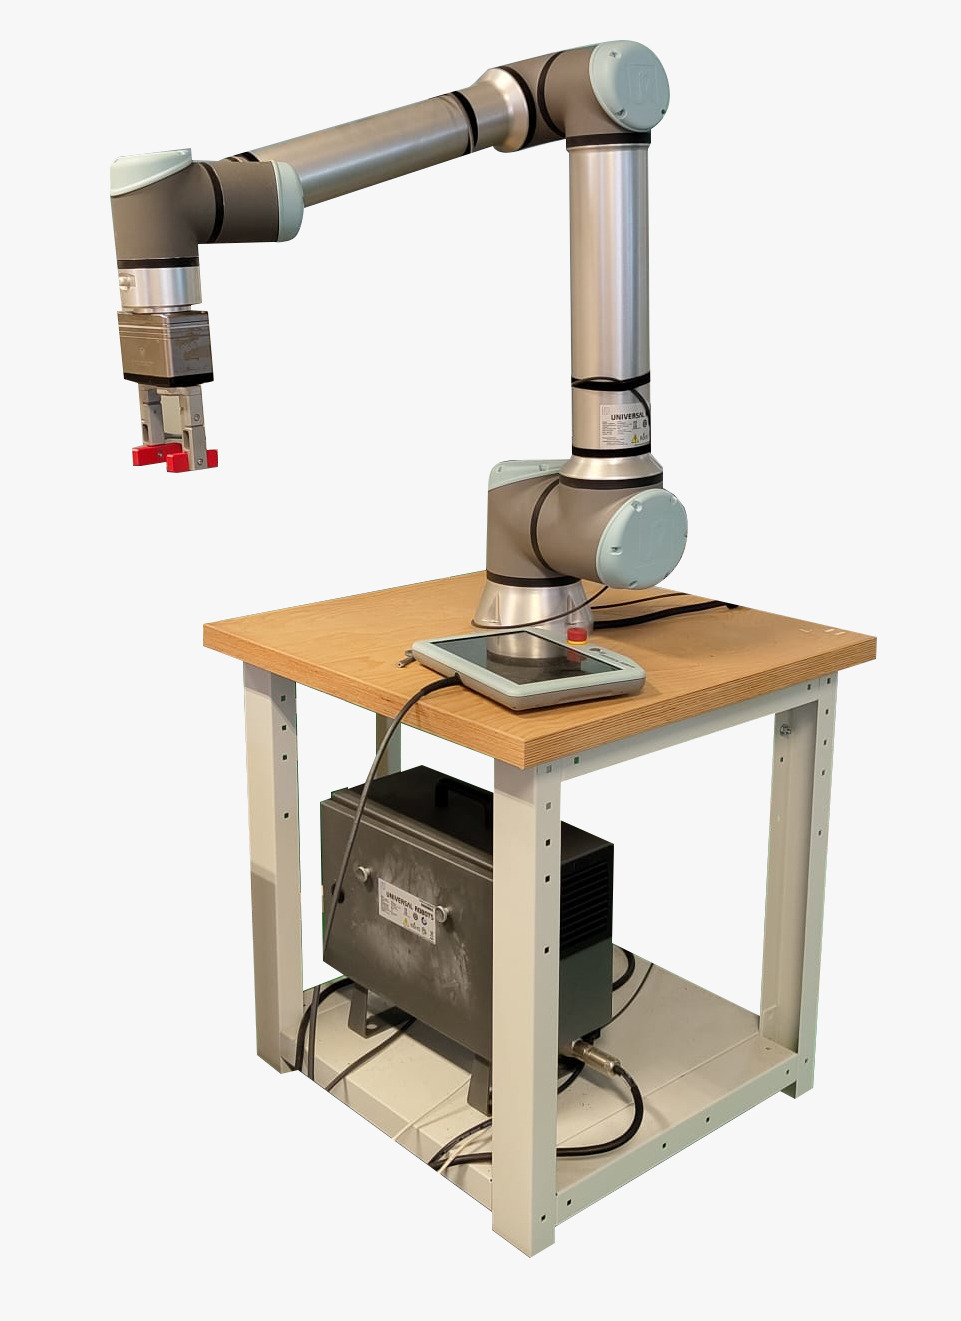
\includegraphics[width=0.4\linewidth]{figs/ur10e.jpeg}
    \caption{UR10e Robot used in the IRIS-LAB, University of Aveiro}
    \label{f:ur10e_iris}
\end{figure}

The UR10e model is one of Universal Robots' most advanced cobots, featuring a payload capacity of 12.5 kg, and a reach of 1300 mm, being designed to automate a wide range of tasks that typically require human input, such as assembly, packaging, and pick-and-place operations~\footnote{UR10e \url{https://www.universal-robots.com/products/ur10-robot/} Accessed: 2024-10-15}.

UR10e's integrated force sensors and collision detection technologies allow to collaborate safely with humans in shared workspaces, making it ideal for \ac{HRC} scenarios. Besides, it offers significant flexibility in terms of programming and adaptability. Its console is intuitive and allows imported pre-programmed scripts, therefore being easily deployed across various industrial tasks with minimal programming experience required by the operator.

This robot, as the core physical entity in this human-robot collaborative system, serves as the dynamic agent for performing collaborative tasks, where its physical attributes were mirrored in an immersive digital environment, regarding the fundamental \ac{DT} concept.

\section{Simulation Environment}

\subsection{Unity}

Unity, developed by Unity Technologies, was selected as the primary platform for developing the \ac{MR} environment in this project. Originally designed for game development, Unity has evolved into a powerful tool for creating interactive 3D applications, including \ac{AR}, \ac{VR}, and \ac{MR}. Its robust architecture and versatility in rendering complex virtual environments make it an ideal choice for building a dynamic \ac{DT} of the UR10e robotic arm. This ability to seamlessly integrate external data sources, such as sensor inputs from real-world hardware, enables a high degree of interactivity and realism in the simulation.

Unity’s \ac{IDE} allows for rapid prototyping and iterative design of both the virtual space and the \ac{MR} user interface. Moreover, the engine's cross-platform compatibility supports a range of devices, including desktop systems and mobile platforms, and can handle real-time rendering of high-fidelity 3D models, essential for \ac{MR} applications. Through the Unity-based simulation, operators can not only control the physical UR10e robot remotely but also visualize real-world tasks in a digital, augmented environment, ensuring accurate synchronization between physical and virtual realms.

In addition, Unity’s robust asset management and scripting support, primarily through C\#, provide developers with the tools to easily simulate complex environments, manage interactive objects, and implement advanced functionality such as collision detection and user input handling. These features enable a realistic and immersive experience for both on-site and remote users, improving the overall effectiveness of the \ac{HRC} system.

% \subsection{Digital Model Implementation of the Robot}

% Here, you can explain how the **Unity URDF Importer package** facilitated the import and management of the robot’s digital model, enabling the creation of a precise digital twin. This section should delve into the **Unity Robotics Hub**, explain why this package was selected, and describe how it contributed to the simulation of the UR10e’s movements and the development of bi-directional communication between the physical and digital environments.


% As introduced in section~\ref{section:Goals}, the primary objective of this dissertation is to explore and implement the concept of Human-Robot Collaboration (\ac{HRC}) by leveraging Mixed Reality (\ac{MR}) technologies. To achieve this goal, a comprehensive framework integrating hardware and software components is designed, facilitating remote collaboration in real-time. This chapter outlines the critical tools used in the implementation of the digital twin, as well as the hardware and software resources required for bi-directional robot control.



\section{Digital Model Implementation of the Robot}
\label{section:digital-model}

\subsection{Digital Robot Model - URDF Importer Package}
In order to correctly mirror the UR10e physical robot model and establish a functional \ac{DT} bidirectional synchronization, the \ac{URDF} model of the robot was imported to Unity simulation environment. Unity Robotics Hub's \ac{URDF} Importer package was used for this very purpose~\footnote{Unity Robotics Hub \url{https://github.com/Unity-Technologies/Unity-Robotics-Hub} Accessed: 2024-02-02}.
This package provided several key advantages during the implementation of the \ac{DT} for the UR10e robot.

The \textit{Unity \ac{URDF} Importer} package significantly facilitated the integration of the \ac{URDF} file, enabling the precise recreation of the UR10e robot's physical structure, including its joints and linkages. This seamless integration supported real-time simulation of the robot's movements and configurations within the Unity environment. Additionally, it allowed the visualization and fine-tuning of physics properties to accurately reflect the robot's real-world dynamics. Essential for bilateral communication between virtual and physical robots, the package also streamlined sensor data import from \ac{ROS}, enhancing the realism of simulations and optimizing development and testing processes.

\section{Pose Registration}
Pose registration is a crucial step in aligning the digital model with the physical robot. In this project, Vuforia, a cutting-edge \ac{AR} software platform, was integrated with Unity to accomplish this alignment.

\subsection{Vuforia}
\label{section:marker-detection}

Vuforia Engine \ac{SDK}, an advanced \ac{AR} development platform that can be used within Unity platform, provides robust capabilities for object recognition and tracking, making it integral to \ac{MR} applications. In this project, Vuforia's image-based tracking system was employed to align the digital model of the robot with its physical counterpart. This was achieved through the detection and tracking of an ArUco marker placed next to the physical robot, ensuring precise spatial alignment between the digital and physical elements within the \ac{MR} environment, thus enhancing real-time interaction accuracy.



% Vuforia offers robust solutions for recognizing and tracking objects in real-world environments, which is crucial in Mixed Reality applications. In this project, Vuforia was used to recognize and track an ArUco marker placed on the physical robot, thus allowing the precise alignment of the digital robot model with its real counterpart.

\subsection{Marker Detection}

An ArUco marker, illustrated in the Figure \ref{f:aruco_marker}, served as a medium to perform accurate pose estimation of the robot within the Unity environment. Besides, the Logitech c922 camera shown in Figure \ref{fig:camera-c922} scanned this marker, enabling the system to overlay the digital model accurately over the physical robot. This ensured precise positioning and manipulation of the digital twin in the \ac{MR} space.

\begin{figure}[h]
    \centering
    \begin{subfigure}[b]{0.45\textwidth}
    \centering
    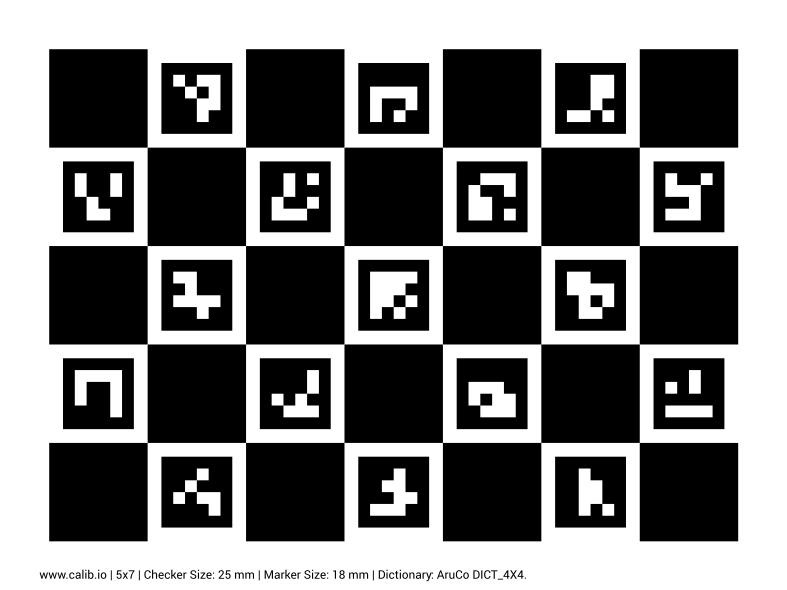
\includegraphics[width=0.7\textwidth]{figs/calib_io_charuco_200x150_5x7_25_18_DICT_4X4.png}
    \caption{ArUco marker for alignment of the digital twin}
    \label{f:aruco_marker}
    \end{subfigure}
        \hfill
    \begin{subfigure}[b]{0.45\textwidth}
        \centering
        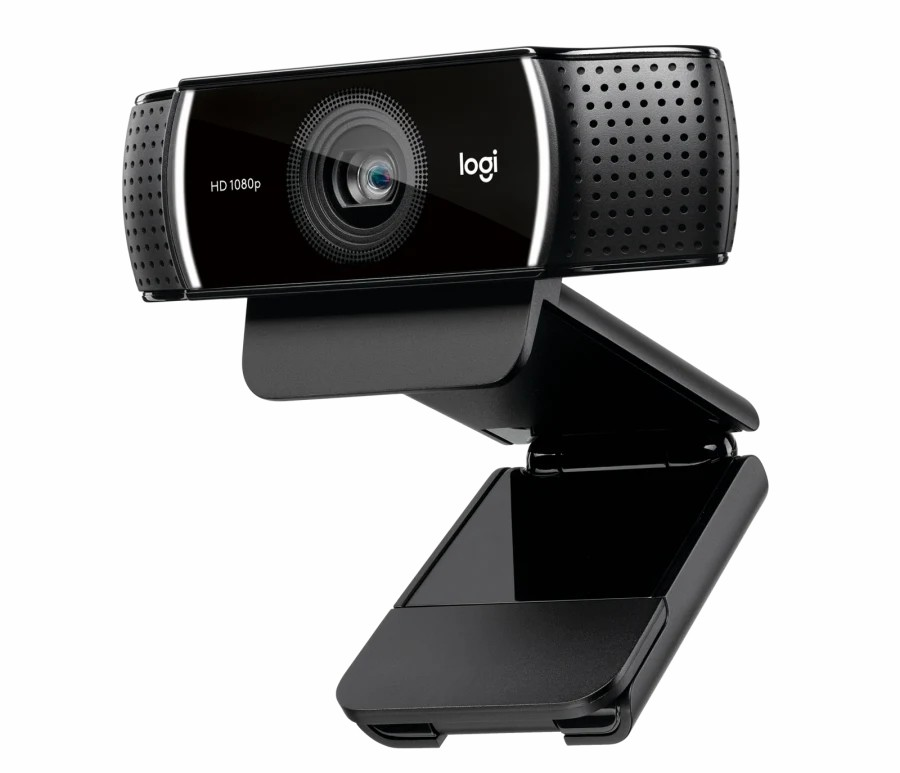
\includegraphics[width=0.7\linewidth]{figs/camera-c922.jpg}
        \caption{Logitech c922 camera used for marker detection}
        \label{fig:camera-c922}
    \end{subfigure}
    \caption{Marker and camera setup for digital and physical robot alignment}
\label{marker-camera}
\end{figure}

In Figure \ref{f:ur10_marker_unity} the digital robot model can be seen positioned realitve to the above described marker.

\begin{figure}[h]
    \centering
    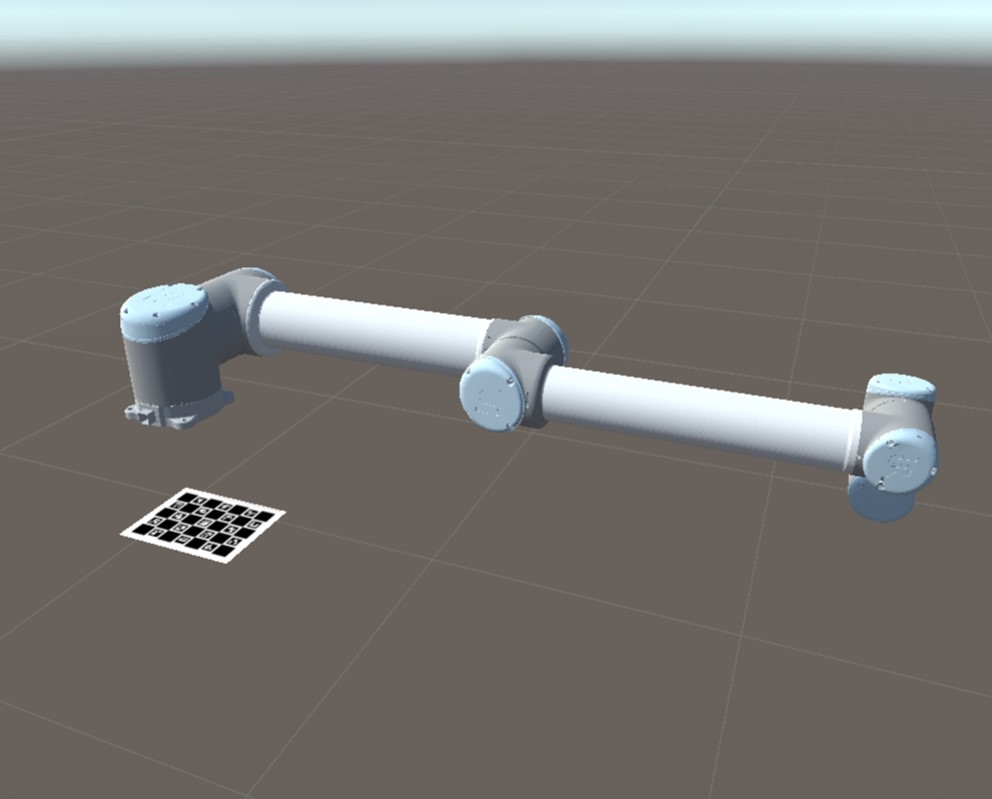
\includegraphics[width=0.6\textwidth]{figs/robot_marker_unity.jpg}
    \caption{Digital UR10 model aligned with ArUco marker in Unity}
    \label{f:ur10_marker_unity}
\end{figure}

* TODO: Add a figure showing the digital UR10 model aligned with the real ArUco marker and the real robot in the background. This will visually represent the alignment process - this figure should be displayed here or in the 4 chapter

\section{Bidirectional Communication}

After having the digital model correctly aligned with the physical robot, the next step was to establish bidirectional communication between the Unity and the UR10e. This communication was essential for enabling remote control of the physical robot through the \ac{DT}, as well as for synchronizing the robot's state between the real and virtual environments.

\subsection{ROS}

The Robot Operating System (\ac{ROS}) was chosen as the middleware for facilitating real-time communication between the physical robot and the Unity environment, since the UR10e robot from IRIS-LAB already had prior developed \ac{ROS} packages, such as \texttt{iris\_ur10e} \footnote{IRIS-LAB github Repository \url{https://github.com/iris-ua/iris_ur10e}, Acessed: 2024-02-02} and \texttt{iris\_sami}~\footnote{IRIS-LAB github Repository for UR10e Robot Manipulation \url{https://github.com/iris-ua/iris_ur10e}, Acessed: 2024-02-02}.

These packages provided a comprehensive \ac{ROS} setup for controlling the UR10e robot, including trajectory planning, RViz visualization, and real-time operation. 
\ac{ROS} offers a robust and flexible framework for developing complex robotic systems. In this project, it enables seamless integration between hardware components and software modules. Specifically, \ac{ROS} facilitates the exchange of sensor data, control commands, and state information between the physical UR10e robot and its digital twin in Unity, ensuring synchronization for remote control and collaborative operations.


% \section{Message Generation}
% \subsection{UR10e ROS Documentation}
% While Unity was chosen for its ability to create immersive environments, ROS (Robot Operating System) was selected to facilitate communication between the physical robot and its digital twin. The UR10e robot runs on ROS Noetic, which was configured on Ubuntu 20.04. By using ROS-TCP-Connector and ROS-TCP-Endpoint packages \footnote{Unity ROS Connector \url{https://github.com/Unity-Technologies/ROS-TCP-Connector} Accessed: 2024-02-02}

% a resume for each definition of the tools used in the implementation of the project - removeeeeeeeeeeeeeeeeeeee?
% Unity serves as the central development platform, integrating 3D models and real-time visualization to create the \ac{DT}. Vuforia, in conjunction with \ac{AR} markers, ensures precise pose registration between the physical robot and its digital counterpart. Additionally, \ac{ROS} (Robot Operating System) serves as the middleware facilitating real-time communication between the physical robot and the Unity environment. Together, these tools form the backbone of the system's functionality, enabling seamless collaboration between human operators and robotic systems in both physical and virtual spaces.
